% Chapter 6
\chapter{Results of the Reproduction}
\label{ch:repro}

This chapter answers RQ1 for the first Lizard model. It uses the LoLCATs recipe of \cref{tab:recipes} and the original Lizard attention.

\section{Runs 0, 1 and 2}
\label{sec:runs}

\textbf{Run 0} was a smoke test with 10 steps in each stage. It passed from the start to the end. The stage 1 validation loss fell from 76.9 to 17.1 in 10 steps, and the job pushed the checkpoints to the Hub.

\textbf{Run 1} was the first full run. Stage 1 finished all 1,178 steps with a best validation loss of 3.2549. Stage 2 then started from a much better model than in the smoke test. Its first validation loss was 5.42 (perplexity 233). After only 10 stage 1 steps, it was 8.85 (perplexity 7,207). Thus stage 1 had a clear effect. At gradient step 386 of stage 2, the forward pass gave NaN, and the job stopped (\cref{sec:nan}).

\textbf{Run 2} repeated stage 2 from the stage 1 checkpoint of Run~1, with the NaN fix. It finished with a validation loss of 2.252 (perplexity approximately 9.5). The \emph{first Lizard model} of this thesis is the stage 1 checkpoint of Run~1 with the stage 2 checkpoint of Run~2.

\section{The scores against the paper and the teacher}
\label{sec:first-scores}

\Cref{tab:first-scores} and \cref{fig:first-scores} compare the first Lizard model with the teacher and with the paper. On all three tasks, the model is clearly below the paper. On PIQA, it is approximately 6.3 SE below the paper, and on ARC-Easy, 10.6 SE. On MMLU, it is 4.8 SE \emph{below} chance.

\begin{table}[ht]
\centering
\small
\caption[Scores of the first Lizard model]{Scores of the first Lizard model (project notes, document~7). Accuracy in \%, with the SE where the harness reports it.}
\label{tab:first-scores}
\begin{tabular}{@{}lrrrrr@{}}
\toprule
Task & \makecell[r]{First Lizard\\model} & \makecell[r]{Teacher,\\this harness} & \makecell[r]{Lizard,\\paper} & \makecell[r]{LoLCATs,\\paper} & \makecell[r]{Teacher,\\paper} \\
\midrule
MMLU, all questions & \textbf{23.3} & 31.7 & 29.8 & 27.3 & 31.0 \\
MMLU subset & 24.9 & 33.7 & -- & -- & -- \\
PIQA & \textbf{68.0} $\pm$ 1.1 & 74.4 $\pm$ 1.0 & 74.8 & 74.6 & 74.1 \\
ARC-Easy & \textbf{54.8} $\pm$ 1.0 & 65.3 $\pm$ 1.0 & 65.6 & 63.0 & 65.4 \\
\bottomrule
\end{tabular}
\end{table}

\begin{figure}[ht]
\centering
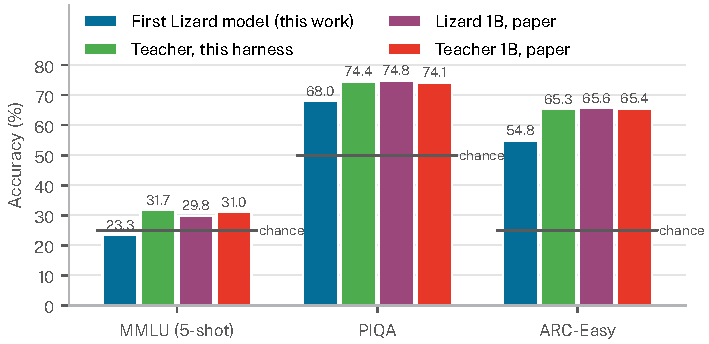
\includegraphics[width=\linewidth]{scores_first_model}
\caption[The first Lizard model against the teacher and the paper]{The first Lizard model against the teacher and the paper. The dark lines show the chance level of each task. Values from \cref{tab:first-scores}.}
\label{fig:first-scores}
\end{figure}

PIQA and ARC-Easy are far above chance (50\% and 25\%). Thus the model still works as a language model. But it is 6.5 points below the teacher on PIQA and 10.5 points on ARC-Easy. The damage is wide. It is not limited to MMLU or to long texts: most PIQA and ARC-Easy prompts are shorter than the 128-token window.

\section{The model selects \enquote{A} on MMLU}
\label{sec:a-collapse}

A score below chance on questions with four options suggests a simple behavior: the model ignores the question and prefers one letter. Then its accuracy in each subject equals the share of that letter among the right answers. \Cref{tab:letters} tests this idea for each letter.

\begin{table}[ht]
\centering
\small
\caption[Accuracy of the first Lizard model against fixed answers]{Accuracy of the first Lizard model against fixed answers on all MMLU questions (\code{letters.py}, project notes, document~7). The real macro mean is 0.233.}
\label{tab:letters}
\begin{tabular}{@{}lrrr@{}}
\toprule
\makecell[l]{If the model\\always gave} & \makecell[r]{Macro\\mean} & \makecell[r]{Mean $|$acc $-$ share$|$\\over subjects} & \makecell[r]{Correlation with\\the accuracy} \\
\midrule
\textbf{\enquote{A}} & \textbf{0.231} & \textbf{0.004} & \textbf{+0.98} \\
\enquote{B} & 0.245 & 0.039 & +0.29 \\
\enquote{C} & 0.254 & 0.051 & $-$0.05 \\
\enquote{D} & 0.270 & 0.087 & $-$0.65 \\
\bottomrule
\end{tabular}
\end{table}

\begin{finding}
On MMLU, the first Lizard model selects \enquote{A} for almost every question. On the MMLU subset, it gives \enquote{A} for 98.6\% of the questions. The accuracy of each subject has a correlation of +0.98 with the share of \enquote{A} as the right answer.
\end{finding}

The question and the four options are usually in the last approximately 100 tokens, inside the window. Thus the collapse is not only a failure of long contexts. The teacher itself is only 6--9 points above chance on MMLU. Thus a model with moderate damage can already fall back to one letter.

\section{The model uses both branches}
\label{sec:ablation}

An earlier idea was that the gated branch did not learn and that the model used only the window. A test removed one branch at inference time and multiplied the other branch by $(1 + \alpha)$. \Cref{tab:ablation} gives the result on PIQA.

\begin{table}[ht]
\centering
\small
\caption[PIQA with one branch removed at inference]{PIQA with one branch removed at inference (\code{ablate.py}, project notes, document~7).}
\label{tab:ablation}
\begin{tabular}{@{}lrr@{}}
\toprule
Model & Accuracy (\%) & Difference \\
\midrule
Full first Lizard model & 67.95 $\pm$ 1.09 & -- \\
Window branch removed: $(1 + \alpha) \cdot$ gated branch & 57.18 $\pm$ 1.15 & $-$10.8 ($z \approx 6.8$) \\
Gated branch removed: $(1 + \alpha) \cdot$ window branch & 52.34 $\pm$ 1.17 & $-$15.6 ($z \approx 9.8$) \\
Chance & 50.0 & \\
\bottomrule
\end{tabular}
\end{table}

Both branches matter. Without the gated branch, the model is almost at chance. This agrees with the design of the paper. Without RoPE, the window cannot find the token order. The gate is the only source of position information. The test measures how much the trained model depends on each branch. It does not show if the architecture needs each branch. The paper tests that question with new training runs (its Table~6).

\section{The gap starts in stage 1}
\label{sec:stage-diff}

The script \code{compare_stages.sh} evaluated the model after stage 1, without LoRA, and after stage 2. \Cref{tab:stage-diff} shows the result. The drop is already present after stage 1. Stage 2 recovers approximately 10 points on PIQA, but MMLU stays near chance. The collapse to \enquote{A} is also present after stage 1. All checkpoints loaded completely: 80 Lizard tensors and 128 LoRA tensors, with 0 missing keys. Thus a loading error does not cause the results.

\begin{table}[ht]
\centering
\small
\caption[The first Lizard model after each stage]{The first Lizard model after each stage (project notes, \enquote{stage difference}).}
\label{tab:stage-diff}
\begin{tabular}{@{}lrrr@{}}
\toprule
Task & After stage 1 & After stage 2 & Teacher \\
\midrule
PIQA & 57.6 $\pm$ 1.2 & 68.0 $\pm$ 1.1 & 74.4 \\
ARC-Easy & 39.0 $\pm$ 1.0 & 54.8 $\pm$ 1.0 & 65.3 \\
MMLU subset & 22.5 (\enquote{A} for 95.4\%) & 24.9 (\enquote{A} for 98.6\%) & 33.7 \\
\bottomrule
\end{tabular}
\end{table}

The gate values give a first explanation. The script measured the gates on one MMLU prompt of 2048 tokens. In layers 1--15, the gate is above 0.999 for all tokens. After 512 tokens, these layers keep at least 95\% of the weight of a token. Thus the gated branch adds up almost all earlier tokens without decay. Only layer 0 has a decay: it keeps 35\% of the weight after 128 tokens. In layer 0, $\alpha$ fell from 1 to 0.042. Thus the window branch of layer 0 has almost no weight. The other layers have $\alpha$ between 0.16 and 0.65. Most sink logits stopped at exact powers of two, such as 0.5, 1.0 and 2.0. This is a sign of bf16 rounding.

\section{The temperature does not change the scores}
\label{sec:temperature}

The harness compares log-likelihoods. A temperature $T$ divides all logits by the same number. This does not change the order of the four letters, so the accuracy must stay the same. \Cref{tab:temperature} confirms this prediction on the stage 1 model.

\begin{table}[ht]
\centering
\small
\caption[The MMLU subset at four temperatures]{The MMLU subset at four temperatures, stage 1 model (project notes, \enquote{temperature}). \enquote{Mass} is the probability of the four letters together. \enquote{Changed} counts the answers that differ from $T = 1$.}
\label{tab:temperature}
\begin{tabular}{@{}rrrrrr@{}}
\toprule
$T$ & Accuracy & \enquote{A} & Changed & Mass & Entropy (bits) \\
\midrule
0.1 & 22.5 & 95.4\% & 0 of 285 & 0.006 & 0.070 \\
0.5 & 22.5 & 95.4\% & 0 of 285 & 0.025 & 0.855 \\
1 & 22.5 & 95.4\% & 0 of 285 & 0.018 & 1.550 \\
2 & 22.5 & 95.4\% & 0 of 285 & 0.002 & 1.879 \\
\bottomrule
\end{tabular}
\end{table}

The test also shows a second problem. The four letters together get only 1.8\% of the probability of the next token at $T = 1$. Thus, for almost all questions, the most probable next token after \enquote{Answer:} is not a letter. The stage 1 model does not follow the answer format of the 5-shot prompt.

\section{Summary of the reproduction}
\label{sec:repro-summary}

\begin{finding}
\textbf{RQ1, first answer.} The first reproduction did not reach the paper. MMLU is 23.3 against 29.8, PIQA 68.0 against 74.8 and ARC-Easy 54.8 against 65.6. The teacher in the same harness gets the expected scores, and the tests of \cref{sec:tests} found no bug. The drop starts in stage 1. On MMLU, the model gives \enquote{A} for almost every question.
\end{finding}
